\documentclass[12pt]{article}

\usepackage{amsmath, mathtools}
\usepackage{amsfonts}
\usepackage{amssymb}
\usepackage{graphicx}
\usepackage{colortbl}
\usepackage{xr}
\usepackage{hyperref}
\usepackage{longtable}
\usepackage{xfrac}
\usepackage{tabularx}
\usepackage{float}
\usepackage{siunitx}
\usepackage{booktabs}
\usepackage{caption}
\usepackage{pdflscape}
\usepackage{afterpage}

\usepackage[round]{natbib}

%\usepackage{refcheck}

\hypersetup{
    bookmarks=true,         % show bookmarks bar?
      colorlinks=true,       % false: boxed links; true: colored links
    linkcolor=red,          % color of internal links (change box color with linkbordercolor)
    citecolor=green,        % color of links to bibliography
    filecolor=magenta,      % color of file links
    urlcolor=cyan           % color of external links
}

%% Comments

\usepackage{color}

\newif\ifcomments\commentstrue

\ifcomments
\newcommand{\authornote}[3]{\textcolor{#1}{[#3 ---#2]}}
\newcommand{\todo}[1]{\textcolor{red}{[TODO: #1]}}
\else
\newcommand{\authornote}[3]{}
\newcommand{\todo}[1]{}
\fi

\newcommand{\wss}[1]{\authornote{blue}{SS}{#1}}
\newcommand{\wpa}[1]{\authornote{magenta}{PA}{#1}}


% For easy change of table widths
\newcommand{\colZwidth}{1.0\textwidth}
\newcommand{\colAwidth}{0.13\textwidth}
\newcommand{\colBwidth}{0.82\textwidth}
\newcommand{\colCwidth}{0.1\textwidth}
\newcommand{\colDwidth}{0.05\textwidth}
\newcommand{\colEwidth}{0.8\textwidth}
\newcommand{\colFwidth}{0.17\textwidth}
\newcommand{\colGwidth}{0.5\textwidth}
\newcommand{\colHwidth}{0.28\textwidth}

% Used so that cross-references have a meaningful prefix
\newcounter{defnum} %Definition Number
\newcommand{\dthedefnum}{GD\thedefnum}
\newcommand{\dref}[1]{GD\ref{#1}}
\newcounter{datadefnum} %Datadefinition Number
\newcommand{\ddthedatadefnum}{DD\thedatadefnum}
\newcommand{\ddref}[1]{DD\ref{#1}}
\newcounter{theorynum} %Theory Number
\newcommand{\tthetheorynum}{T\thetheorynum}
\newcommand{\tref}[1]{T\ref{#1}}
\newcounter{tablenum} %Table Number
\newcommand{\tbthetablenum}{T\thetablenum}
\newcommand{\tbref}[1]{TB\ref{#1}}
\newcounter{assumpnum} %Assumption Number
\newcommand{\atheassumpnum}{P\theassumpnum}
\newcommand{\aref}[1]{A\ref{#1}}
\newcounter{goalnum} %Goal Number
\newcommand{\gthegoalnum}{P\thegoalnum}
\newcommand{\gsref}[1]{GS\ref{#1}}
\newcounter{instnum} %Instance Number
\newcommand{\itheinstnum}{IM\theinstnum}
\newcommand{\iref}[1]{IM\ref{#1}}
\newcounter{reqnum} %Requirement Number
\newcommand{\rthereqnum}{P\thereqnum}
\newcommand{\rref}[1]{R\ref{#1}}
\newcounter{lcnum} %Likely change number
\newcommand{\lthelcnum}{LC\thelcnum}
\newcommand{\lcref}[1]{LC\ref{#1}}
\newcounter{calcnum} %Calculation Number
\newcommand{\cthecalcnum}{C\thecalcnum}
\newcommand{\cref}[1]{C\ref{#1}}
\newcounter{outputnum} %Output Number
\newcommand{\otheoutputnum}{O\theoutputnum}
\newcommand{\oref}[1]{O\ref{#1}}
\newcounter{bibnum} %Output Number
\newcommand{\bthebibnum}{\thebibnum}
\newcommand{\bref}[1]{\ref{#1}}


\newcommand{\famname}{LODES} % PUT YOUR PROGRAM NAME HERE
\newcommand{\famdesc}{Library of ODE Solvers}

\usepackage{fullpage}

\begin{document}

\title{Commonality Analysis for a \famdesc{} (\famname{})} 
\author{Paul Aoanan}
\date{\today}

\maketitle

~\newpage

\pagenumbering{roman}

\section{Revision History}

\begin{tabularx}{\textwidth}{p{3cm}p{2cm}X}
\toprule {\bf Date} & {\bf Version} & {\bf Notes}\\
\midrule
\today & 1.0 & Initial Draft.\\
%Date 2 & 1.1 & Notes\\
\bottomrule
\end{tabularx}

~\newpage
	
\section{Reference Material}

This section records information for easy reference.

\subsection{Table of Units}

This section does not apply to this program family.

\subsection{Table of Symbols}

The table that follows summarizes the symbols used in this document along with
their units.  The choice of symbols was made to be consistent with the numeral analysis
and ordinary differential equation literature and with existing documentation
for solving ordinary differential equations.  The symbols are listed in alphabetical order.

\renewcommand{\arraystretch}{1.2}
%\noindent \begin{tabularx}{1.0\textwidth}{l l X}
\noindent \begin{longtable*}{l l p{12cm}} \toprule
\textbf{symbol} & \textbf{unit} & \textbf{description}\\
\midrule
$dy/dx$ & \text {-} & rate of change of $y$ with respect to $x$\\
$f(x, y)$ & \text{-} & Explicit form of the ODE function containing $(x,y)$\\
$f_{x}(x, y)$ & \text{-} & Explicit form of the derivative of $f(x, y)$ with respect to x\\
$f_{y}(x, y)$ & \text{-} & Explicit form of the derivative of $f(x, y)$ with respect to y\\
$h$ & \text{-} & step-size from $x_\text{(0)}$ to the next point $x_\text{(1)}$, where $x_\text{(1)} = x_\text{(0)} + h$\\
$K_1, K_2, K_3, K_4$ & \text{-} & Intermediary variables used in the Runge-Kutta method\\
$n$ & \text{-} & reference recursion step\\
$o$ & \text{-} & solution variable\\
$x_\text{0}$ & \text{-} & Initial value $x$\\
$x_\text{k}$ & \text{-} & Final value $x$\\
$x_\text{n}$ & \text{-} & Intermediate $n^\text{th}$ value $x$\\
$y_\text{0}$ & \text{-} & Initial value $y$\\ 
$y_\text{k}$ & \text{-} & Final value $y$\\
$y_\text{n}$ & \text{-} & Intermediate $n^\text{th}$ value $y$\\ 
$y'$ & \text{-} & Implicit form of the first order ODE = $f(x, y)$\\
$y^\text{(n)}$ & \text{-} & Implicit form of the ODE to the $n^\text{th}$ order\\
\bottomrule
\end{longtable*}

\subsection{Abbreviations and Acronyms}

\renewcommand{\arraystretch}{1.2}
\begin{tabular}{l l} 
  \toprule		
  \textbf{symbol} & \textbf{description}\\
  \midrule 
  A & Assumption\\
  C & Calculation\\
  DD & Data Definition\\
  %GD & General Definition\\
  GS & Goal Statement\\
  IM & Instance Model\\
  IVP & Initial Value Problem\\
  %LC & Likely Change\\
  ODE & Ordinary Differential Equation\\
  PS & Physical System Description\\
  %R & Requirement\\
  SRS & Software Requirements Specification\\
  \famname{} & \famdesc{}\\
  T & Theoretical Model\\
  O & Output\\
  \bottomrule
\end{tabular}\\

\newpage

\tableofcontents

~\newpage

\pagenumbering{arabic}

\section{Introduction}

%\wss{This CA template is based on \citet{Smith2006}.

In physical sciences, mathematical models are derived from scientific models to
represent a real world phenomenon through formal mathematical constructs.

Scientific models in the study of radioactivity, carbon decay, and Newton's Law of Cooling
involve the use of ordinary differential equations (ODEs).

Known elementary techniques of solving ODEs in the discrete domain use the linear approximation
method wherein the solution is based upon assuming or ``approximating" the slope of the tangent
line from one reference point to the next until the target point has been reached.

The following section provides an overview of the Commonality Analysis (CA) for a
program family of ODE solvers for Initial Value Problems (IVP). The developed program will be
called \famdesc{} (\famname{}). This section explains the purpose of this
document, the scope of the family, the characteristics of the intended readers,
and the organization of the document.

\subsection{Purpose of Document}
The main purpose of this document is to formally describe program families of
the known well-known methods of solving Initial Value Problems of ODEs.
The goals and mathematical models used in the \famname{} code are provided with
an emphasis on explicitly identifying assumptions, constraints, and unambiguous definitions.

This document contains the description of the functionalities of the \famname{} software
library. This document is the starting point for the subsequent software development
activities, including writing the requirements specification, design specification, code,
software verification, validation plan, and execution.

\subsection{Scope of the Family}
The scope of the family is limited to the library of IVP ODE solvers. Given
the appropriate inputs, each program in \famname{} is intended to find the solution to an
Initial Value ODE problem.

\subsection{Characteristics of Intended Reader}
Reviewers of this document should have an elementary understanding of ordinary differential
equations and numerical methods, as typically covered in first and second year Calculus courses.
The users of \famname{} can have a lower level expertise, as explained in
Section~\ref{SecUserCharacteristics}.

\subsection{Organization of Document}
The organization of this document follows the template for a CA for scientific
computing software proposed by~\cite{Smith2006}. The presentation follows the standard
pattern of presenting goals, theories, definitions, and assumptions.
For a bottom-up approach, readers can begin reviewing the instance models in
Section \ref{sec_instance} and trace back to review additional information required.
The instance models provide the methods to solve Initial Value Problems (IVP)
of Ordinary Differential Equations (ODEs).

\section{General System Description}

This section identifies the interfaces between the system and its environment,
describes the potential user characteristics and lists the potential system
constraints.

\subsection{Potential System Contexts}

Figure~\ref{Fig_SystemContext} shows the system context.  A circle represents an
external entity outside the software, the driver program in this case. The driver program
shall use \famname{} in solving the ODE Initial Value Problems (IVPs).
A rectangle represents the software system itself (\famname{}). 
Arrows are used to show the data flow between the system and its environment.

\begin{figure}[h!]
\begin{center}
 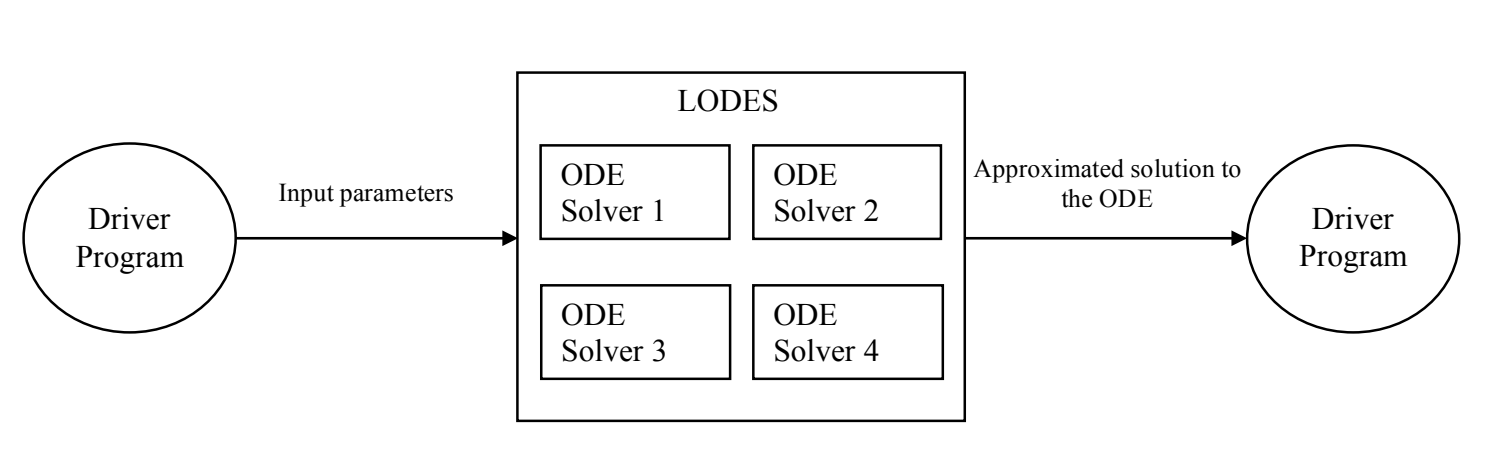
\includegraphics[width=0.9\textwidth, height=0.20\textheight]{SystemContextFigure}
\caption{System Context}
\label{Fig_SystemContext} 
\end{center}
\end{figure}

Programs in \famname{} are used inside a driver program.  The external interaction is through
program calls. The solution to the ODE IVP is the output of the function. 
The responsibilities of the user and the system are as follows:

\begin{itemize}
\item User Responsibilities:
\begin{itemize}
\item Provide the correct program call, while adhering to conventions of the program's prototype
\item Provide the input details of the ODE to be solved, ensuring no errors in data entry
\item Declaration of the ODE method to be used in solving the ODE
\item Provide a valid ODE function which assumes a first order continuous ODE
\end{itemize}
\item \famname{} Responsibilities:
\begin{itemize}
\item Detect an improper input, such as invalid characters in the ODE statement and incomplete input arguments
\item Parse the input ODE string into a meaningful ODE equation that can be manipulated by the machine
\item Detect a data type mismatch where applicable, such as a string of characters in a floating point argument
\item Calculate the solution to the ODE problem
\item Provide the user access to the outputs of the program
\end{itemize}
\end{itemize}

\subsection{Potential User Characteristics} \label{SecUserCharacteristics}

The end user of \famname{} should have at least some basic programming experience and
an understanding of undergraduate Level 1 Calculus.

\subsection{Potential System Constraints}

There are no system constraints applicable.

\section{Commonalities}
This section primarily presents the background and motivation of the program family, which gives a
high-level view of the problem to be solved.  This is followed by the terminologies used, data
definitions, goals of the software, and the theoretical models used. 
% solution characteristics
% specification, which presents the theories, definitions, assumptions, and finally
% the instance models as variabilities.

\subsection{Background Overview} \label{Sec_Background}
\famname{} is a software library developed to be provide a means to solve Initial Value
Problems for ODEs using numerical methods. It can be used to solve different variations of ODEs
given their initial values. It can be implemented to find the most accurate method (the method
which produces the least error in their scientific computing implementation).

\subsection{Terminology and  Definitions}

This subsection provides a list of terms that are used in the subsequent
sections and their meanings, with the purpose of reducing ambiguity and making it
easier to correctly understand the requirements:

\begin{itemize}

\item Initial values: ``starting point" ($x_\text{0}, y_\text{0}$) of known values that
exists in the domain of the solution

\item Final values: An ``ending point" ($x_\text{k}, y_\text{k}$) of unknown value $y_\text{k}$
that exists in the domain of the solution

\item Step size: The measure of arbitrary positive value ($h$) from the starting point
($x_\text{0}, y_\text{0}$) of the domain to the next ($x_\text{1}, y_\text{1}$), where
$x_\text{1} = x_\text{0} + h$

\item Derivative: The amount by which a a function changes at any given point as an
instantaneous rate of change

\item Numerical Analysis: A branch of mathematics and computer science wherein the solutions
are numerical approximations taking into account the errors involved in the process.

\item Numerical Approximation: An approximation of the exact solution to the problem with the
use of known numerical techniques while minimizing error.

\item Recursion: The repeated application of a procedure or program.

\item Initial Value Problem: A type of ODE problem where the initial conditions are stated and
used to find the solution to the ODE.

\item Linear Function: A function which graph is a straight line.

\item Continuous Function: A function which does not have any breaks in its graph across its domain.

\end{itemize}

\subsection{Data Definitions} \label{sec_datadef}

This section collects and defines all the data needed to build the instance
models. The dimension of each quantity is also given.

~\newline

\noindent
\begin{minipage}{\textwidth}
\renewcommand*{\arraystretch}{1.5}
\begin{tabular}{| p{\colAwidth} | p{\colBwidth}|}
\hline
\rowcolor[gray]{0.9}
Number& DD\refstepcounter{datadefnum}\thedatadefnum \label{D_SLOPE}\\
\hline
Label& \bf Slope of the Tangent Line to a Curve\\
\hline
Symbol &$dy/dx$\\
\hline
% Units& $Mt^{-3}$\\
% \hline
  %Equation&$\frac{dy}{dx} = (y_{n+1} - y_n) / (x_{n+1} - x_n)$, of a function $y(x)$\\
  Equation&$dy/dx = $ $\lim_{h\to{0}} \frac{y(x+h) - y(x)}{h}$\\
  \hline
  Description 
        &$dy/dx$ is the slope of the tangent line to $y(x)$.\\
        &$dy/dx$ can be denoted as $y'(x)$ or $f(x, y$). [\tref{T_ODE}]\\
        &$h$ is the step size.\\
  \hline
  Source&
        Nagle, et al, "Solutions and Initial Value Problems," in
        \textit{Fundamentals of Differential Equations and Boundary Value Problems},
        3rd ed. USA: Addison Wesley Longman, 2000, ch. 1, p. 7. ~\cite{Nagle2000}
  \\
  \hline
  Ref.\ By & \iref{euler}, \iref{trapezoid}, \iref{heun}, \iref{runge}\\
  \hline
\end{tabular}
\end{minipage}\\

\subsection{Goal Statements}

\begin{itemize}

\item[GS\refstepcounter{goalnum}\thegoalnum \label{G_SolveForY}:]{
Given an explicit first order continuous ordinary differential equation (ODE) problem
represented by $y'= f(x,y)$, the set of initial
values $x_\text{0}$ and $y_\text{0}$ that satisfy $y(x_\text{0}) = y_\text{0}$,
and $x_\text{k}$, return $y_\text{k}$ such that $y(x_\text{k}) = y_\text{k}$ (the final
values), where $y(x)$ is a function, $f(x,y)$ is a function, and $x$
is an independent variable.}

% \item[GS\refstepcounter{goalnum}\thegoalnum \label{G_InputOutput}:]{
% Provide the user the means of providing the required inputs, calling the ODE solver
% program, and returning the results.}

\end{itemize}

\subsection{Theoretical Models} \label{sec_theoretical}

This section focuses on the general equations and laws that \famname{} is based
on.

~\newline

\noindent
\begin{minipage}{\textwidth}
\renewcommand*{\arraystretch}{1.5}
\begin{tabular}{| p{\colAwidth} | p{\colBwidth}|}
  \hline
  \rowcolor[gray]{0.9}
  Number& T\refstepcounter{theorynum}\thetheorynum \label{T_ODE}\\
  \hline
  Label&\bf Initial Value Problem (IVP) of First Order Ordinary Differential Equation (ODE)\\
  \hline
  Equation& Implicit form of the first order ODE:\\%$n^{th}$ order ODE:\\
  &$f(x, y, y') = o$\\ %, y',...y^\text{(n)}) = o$\\
  &Explicit form of the first order ODE:\\ %$n^{th}$ order ODE:\\ 
  &$y' = f(x, y)$\\
  %&$y^\text{(n)} = f(x, y, y',..., y^\text{(n-1)})$\\
  &Given the initial values:\\
  &$(x_0, y_0)$ such that $y(x_0) = y_0$,\\
  &Find $y_k$ such that $y(x_k) = y_k$.\\
  %Equation&  $y^{(n)} = F(x,y,y',...,y^{(n-1)})$\\ %; y(x_\text{0}) = y_\text{0}$\\
  \hline
  Description & 
                The above model gives the definition of an ordinary differential equation initial
                value problem.

                A differential equation is an equation, where the unknown is a
                function and both the function and its derivatives (rate of change) appear in the
                equation.

                An ordinary differential equation is a differential equation involving only ordinary derivatives with respect to a single independent variable.

                For an arbitrary ODE, the true solution will, in general, be unknown.

                Using the given initial values, numerical methods are used to find numerical approximations of the solution to the ODE. 
                \\
  \hline
  Source &
           M. Heath, "Ordinary Differential Equations," in \textit{Scientific Computing an
           Introductory Survey, 2}nd ed. New York: McGraw Hill, 2002, ch. 9.1, pp. 383 - 384.
           ~\cite{Heath2002} 
           \\
  % The above web link should be replaced with a proper citation to a publication
  \hline
  Ref.\ By & \ddref{D_SLOPE}, \tref{T_uniqsoln}, \iref{euler}, \iref{trapezoid}, \iref{heun},
  \iref{runge}, \aref{A_typeoff}, \aref{A_explicit}, \aref{A_linearity},
  \aref{A_continuous}, \aref{A_roots}, \aref{A_boundary}, \aref{A_entriesofh}, 
  \aref{A_entriesofx0}, \aref{A_dimofx0}, \aref{A_entriesofy0}, \aref{A_dimofy0},
  \aref{A_entriesofxk}, \aref{A_dimofxk}, \oref{O_valuesyk}\\
  \hline
\end{tabular}
\end{minipage}\\

~\newline

\noindent
\begin{minipage}{\textwidth}
\renewcommand*{\arraystretch}{1.5}
\begin{tabular}{| p{\colAwidth} | p{\colBwidth}|}
  \hline
  \rowcolor[gray]{0.9}
  Number& T\refstepcounter{theorynum}\thetheorynum \label{T_uniqsoln}\\
  \hline
  Label&\bf Existence and Uniqueness of the Solution\\
  \hline
  Equations&  $y' = f(x,y)$ [\tref{T_ODE}]
  ~\newline
  $y(x_\text{0}) = y_\text{0}$
  ~\newline
  Assuming $f$ and $y'$ are continuous in $R = \{(x,y): a < x < b, c < y < d\}$, where R is a rectangle
  and $a, b, c, d$ are its vertices
  ~\newline
  The initial value problem has a unique solution in some interval
  ~\newline
  $x_\text{0} - h < x < x_\text{0} + h$\\
  %Equation&  $y^{(n)} = F(x,y,y',...,y^{(n-1)})$\\ %; y(x_\text{0}) = y_\text{0}$\\
  \hline
  Description & 
                The above theoretical model shows that when an equation satisfies the initial values,
                it is assured that a solution to the initial value problem exists. It is desirable to know
                whether or not the equation has an existing solution before effort is made to solve it.
                As well, the theoretical model states that if a solution is found, then it is the only solution to
                the initial value problem. 
                \\
  \hline
  Source &
           Nagle, et al, "Solutions and Initial Value Problems," in
           \textit{Fundamentals of Differential Equations and Boundary Value Problems},
           3rd ed. USA: Addison Wesley Longman, 2000, ch. 1, p. 12. ~\cite{Nagle2000}
           \\
  % The above web link should be replaced with a proper citation to a publication
  \hline
  Ref.\ By & \iref{euler}, \iref{trapezoid}, \iref{heun}, \iref{runge},
  \aref{A_continuous}, \aref{A_roots}, \aref{A_boundary}, \aref{A_entriesofh}, 
  \aref{A_entriesofx0}, \aref{A_dimofx0}, \aref{A_entriesofy0}, \aref{A_dimofy0},
  \aref{A_entriesofxk}, \aref{A_dimofxk}, \oref{O_valuesyk}\\
  \hline
\end{tabular}
\end{minipage}\\

~\newline

\section{Variabilities}
This section presents the variabilities in \famname{}. It details the varying instance models,
gives the assumptions for the input, the variabilities in the calculations, and
finally the target output.

\subsection{Instance Models} \label{sec_instance}    

This section transforms the problem defined in Section~\ref{Sec_Background} into 
one which is expressed in mathematical terms. It uses concrete symbols defined 
in Section~\ref{sec_theoretical}.

~\newline

%Instance Model 1

\noindent
\begin{minipage}{\textwidth}
\renewcommand*{\arraystretch}{1.5}
\begin{tabular}{| p{\colAwidth} | p{\colBwidth}|}
  \hline
  \rowcolor[gray]{0.9}
  Number& IM\refstepcounter{instnum}\theinstnum \label{euler}\\
  \hline
  Label& \bf Euler's Method of Finding the Solution to an ODE IVP\\
  \hline
  Input& $f(x,y), h, x_\text{0}, y_\text{0}, x_\text{k}$\\
  \hline
  Output& $y_\text{k}$ such that $y_\text{k} = y(x_\text{k})$  \\
  &using the recursive formulas:\\
  &$x_\text{n+1} = x_\text{n} + h, n = 0, 1, 2,...$\\
  &$y_\text{n+1} = y_\text{n} + h*f(x_\text{n}, y_\text{n}), n = 0, 1, 2,...$\\
  \hline
  Description&$y' = f(x, y)$ is the first order ODE.\\
  &$h$ is the constant step size.\\
  &$x_\text{0}$ is the initial value of $x$.\\
  &$x_\text{n+1}$ is the value of $x$ in the next equation iteration.\\
  &$x_\text{k}$ is the final value of $x$.\\
  &$y_\text{0}$ is the initial value of $y$, such that $y_\text{0} = y(x_\text{0})$.\\
  &$y_\text{n+1}$ is the value of $y$ in the next equation iteration.\\
  &$y_\text{k}$ is the final value of $y$.\\
  &$n$ is the reference recursion step.\\

  & The above equations are used recursively until $x_\text{n+1} = x_\text{k}$ and $y_\text{n+1} = y_\text{k}$.
  \\
  \hline
  Sources&
        Nagle, et al, "The Approximation Method of Euler," in
        \textit{Fundamentals of Differential Equations and Boundary Value Problems,
        3}rd ed. USA: Addison Wesley Longman, 2000, ch. 1, sec. 1.5, pp. 31-32. ~\cite{Nagle2000}
  \\
  \hline
  Ref.\ By & \iref{heun}, \iref{trapezoid}, \aref{A_programcalls},
  \aref{A_typeoff}, \aref{A_explicit}, \aref{A_linearity},
  \aref{A_continuous}, \aref{A_roots}, \aref{A_boundary}, \aref{A_entriesofh}, 
  \aref{A_entriesofx0}, \aref{A_dimofx0}, \aref{A_entriesofy0}, \aref{A_dimofy0},
  \aref{A_entriesofxk}, \aref{A_dimofxk}

  \\
  \hline
\end{tabular}
\end{minipage}\\

\subsubsection*{Detailed derivation of Euler's Method}

Let $y' = f(x, y),$   $y(x_0) = y_0$, $h$ as a fixed positive number
(step-size), and consider the equally spaced points in the domain:\\
\\
\hspace*{2ex} $x_n = x_0 + nh,$   $n = 0, 1, 2...$\\
\\
The construction of values $y_n$ that approximate the solution values proceeds as follows.
At the point $(x_0, y_0)$, the slope of the solution to $y' = f(x, y)$ is given by
${dy}/{dx} = f(x_0, y_0)$. Hence the tangent line to the solution curve at the initial point is:\\
\\
\hspace*{2ex} $y = y_0 + (x - x_0)*f(x_0, y_0)$.\\
\\
Using this tangent line to approximate the next point in the solution set, we find that
for the point $x_1 = x_0 + h$, we can assume the following approximation:\\
\\
\hspace*{2ex} $y_1 = y_0 + h*f(x_0, y_0).$\\
\\
Repeating the process (recursion), until we reach $y_k$ yields the derivation of Euler's Method.

~\newline

%Instance Model 2

\noindent
\begin{minipage}{\textwidth}
\renewcommand*{\arraystretch}{1.5}
\begin{tabular}{| p{\colAwidth} | p{\colBwidth}|}
  \hline
  \rowcolor[gray]{0.9}
  Number& IM\refstepcounter{instnum}\theinstnum \label{trapezoid}\\
  \hline
  Label& \bf Trapezoid Method of Finding the Solution to an ODE IVP\\
  \hline
  Input& $f(x,y), h, x_\text{0}, y_\text{0}, x_\text{k}$\\
  \hline
  Output& $y_\text{k}$ such that $y_\text{k} = y(x_\text{k})$  \\
  &using the recursive formulas:\\
  &$x_\text{n+1} = x_\text{n} + h, n = 0, 1, 2,...$\\
  &$y_\text{n+1} = y_\text{n} + h*[f(x_\text{n}, y_\text{n})+f(x_\text{n+1}, y_\text{n+1})] / 2,
  n = 0, 1, 2,...$\\
  \hline
  Description&$y' = f(x, y)$ is the first order ODE.\\
  &$h$ is the constant step size.\\
  &$x_\text{0}$ is the initial value of $x$.\\
  &$x_\text{n+1}$ is the value of $x$ in the next equation iteration.\\
  &$x_\text{k}$ is the final value of $x$.\\
  &$y_\text{0}$ is the initial value of $y$, such that $y_\text{0} = y(x_\text{0})$.\\
  &$y_\text{n+1}$ is the value of $y$ in the next equation iteration.\\
  &$y_\text{k}$ is the final value of $y$.\\
  &$n$ is the reference recursion step.\\

  & The above equations are used recursively until $x_\text{n+1} = x_\text{k}$ and $y_\text{n+1} = y_\text{k}$.
  \\
  \hline
  Sources&
        M. Heath, "Numerical Solution of ODEs," in \textit{Scientific Computing an
        Introductory Survey, 2}nd ed. New York: McGraw Hill, 2002, ch. 9.3, p. 399 - 400.
        ~\cite{Heath2002} 
  \\
  \hline
  Ref.\ By & \aref{A_programcalls},
  \aref{A_typeoff}, \aref{A_explicit}, \aref{A_linearity},
  \aref{A_continuous}, \aref{A_roots}, \aref{A_boundary}, \aref{A_entriesofh}, 
  \aref{A_entriesofx0}, \aref{A_dimofx0}, \aref{A_entriesofy0}, \aref{A_dimofy0},
  \aref{A_entriesofxk}, \aref{A_dimofxk}
  \\
  \hline
\end{tabular}
\end{minipage}\\

\subsubsection*{Detailed derivation of the Trapezoid Method}

Using [\iref{euler}] as a starting point:\\
\\
\hspace*{2ex}$x_\text{n+1} = x_\text{n} + h, n = 0, 1, 2,...$\\
\hspace*{2ex}$y_\text{n+1} = y_\text{n} + h*f(x_\text{n}, y_\text{n}), n = 0, 1, 2,...$\\
\\
The Reverse Euler's Method can be derived by taking the values at the next iteration point
while working backwards:\\
\\
\hspace*{2ex}$x_\text{n+1} = x_\text{n} + h, n = 0, 1, 2,...$\\
\hspace*{2ex}$y_\text{n+1} = y_\text{n} + h*f(x_\text{n+1}, y_\text{n+1}), n = 0, 1, 2,...$\\
\\
Using a trapezoid formed by the two approximations, the average can be combined into the
trapezoid method:\\
\\
\hspace*{2ex}$x_\text{n+1} = x_\text{n} + h, n = 0, 1, 2,...$\\
\hspace*{2ex}$y_\text{n+1} = y_\text{n} + h*[f(x_\text{n}, y_\text{n})+f(x_\text{n+1},
y_\text{n+1})] / 2, n = 0, 1, 2,...$\\
\\
Repeating the process (recursion) until we reach $y_k$ yields the Trapezoid Method.\\

~\newline

%Instance Model 3

\noindent
\begin{minipage}{\textwidth}
\renewcommand*{\arraystretch}{1.5}
\begin{tabular}{| p{\colAwidth} | p{\colBwidth}|}
  \hline
  \rowcolor[gray]{0.9}
  Number& IM\refstepcounter{instnum}\theinstnum \label{heun}\\
  \hline
  Label& \bf Heun's Method of Finding the Solution to an ODE IVP\\
  \hline
  Input& $f(x,y), h, x_\text{0}, y_\text{0}, x_\text{k}$\\
  \hline
  Output& $y_\text{k}$ such that $y_\text{k} = y(x_\text{k})$  \\
  &using the recursive formulas:\\
  &$x_\text{n+1} = x_\text{n} + h, n = 0, 1, 2,...$\\
  &$y_\text{n+1} = y_\text{n} + \frac{h}{2}\{[f(x_n, y_n) + f(x_n + h, y_n + h*f(x_n, y_n)]\}, n = 0, 1, 2,...$\\
  \hline
  Description&$y' = f(x, y)$ is the first order ODE.\\
  &$h$ is the constant step size.\\
  &$x_\text{0}$ is the initial value of $x$.\\
  &$x_\text{n+1}$ is the value of $x$ in the next equation iteration.\\
  &$x_\text{k}$ is the final value of $x$.\\
  &$y_\text{0}$ is the initial value of $y$, such that $y_\text{0} = y(x_\text{0})$.\\
  &$y_\text{n+1}$ is the value of $y$ in the next equation iteration.\\
  &$y_\text{k}$ is the final value of $y$.\\
  &$n$ is the reference recursion step.\\

  & The above equations are used recursively until $x_\text{n+1} = x_\text{k}$ and $y_\text{n+1} = y_\text{k}$.
  \\
  \hline
  Sources&
        Nagle, et al, "Improved Euler's Method," in
        \textit{Fundamentals of Differential Equations and Boundary Value Problems},
        3rd ed. USA: Addison Wesley Longman, 2000, ch. 3, sec. 3.5, pp. 124-129. ~\cite{Nagle2000}
  \\
  \hline
  Ref.\ By & \aref{A_programcalls},
  \aref{A_typeoff}, \aref{A_explicit}, \aref{A_linearity},
  \aref{A_continuous}, \aref{A_roots}, \aref{A_boundary}, \aref{A_entriesofh}, 
  \aref{A_entriesofx0}, \aref{A_dimofx0}, \aref{A_entriesofy0}, \aref{A_dimofy0},
  \aref{A_entriesofxk}, \aref{A_dimofxk}

  \\
  \hline
\end{tabular}
\end{minipage}

\newpage

\subsubsection*{Detailed Derivation of Heun's Method}

By modifying the trapezoid scheme [\iref{trapezoid}]:\\
\\
\hspace*{2ex}$x_\text{n+1} = x_\text{n} + h, n = 0, 1, 2,...$\\
\hspace*{2ex}$y_\text{n+1} = y_\text{n} + h*[f(x_\text{n}, y_\text{n})+f(x_\text{n+1},
y_\text{n+1})] / 2, n = 0, 1, 2,...$\\
\\
by using a predicted approximation for $y_{n+1} = y_n + h * f(x_n, y_n)$, we can derive:\\
\\
\hspace*{2ex}$x_\text{n+1} = x_\text{n} + h, n = 0, 1, 2,...$\\
\hspace*{2ex}$y_\text{n+1} = y_\text{n} + \frac{h}{2}\{[f(x_n, y_n) + f(x_n + h, y_n + h*f(x_n, y_n)]\}, n = 0, 1, 2,...$\\
\\
Repeating the process (recursion) until we reach $y_k$ yields Heun's Method.\\

~\newline

% %Instance Model 3

% \noindent
% \begin{minipage}{\textwidth}
% \renewcommand*{\arraystretch}{1.5}
% \begin{tabular}{| p{\colAwidth} | p{\colBwidth}|}
%   \hline
%   \rowcolor[gray]{0.9}
%   Number& IM\refstepcounter{instnum}\theinstnum \label{taylor}\\
%   \hline
%   Label& \bf Second Order Taylor Series Method of Finding the Solution to an ODE IVP\\
%   \hline
%   Input& $y' = f(x,y), h, x_\text{0}, y_\text{0}, x_\text{k}$\\
%   \hline
%   Output& $y_\text{k}$ such that $y_\text{k} = y(x_\text{k})$  \\
%   &by first differentiating $f(x, y)$ to obtain:\\
%   &$y'' = f_{x}(x, y) + f_{y}(x, y)*f(x, y)$.\\
%   &using the recursive formulas:\\
%   &$x_\text{n+1} = x_\text{n} + h, n = 0, 1, 2,...$\\
%   &$y_\text{n+1} = y_\text{n} + h * f(x,y) + \frac{h^2}{2}*(f_{x}(x, y) + f_{y}(x, y)*f(x, y)), n = 0, 1, 2,...$\\
%   \hline
%   Description&$y' = f(x, y)$ is the first order ODE.\\
%   &$h$ is the constant step size.\\
%   &$x_\text{0}$ is the initial value of $x$.\\
%   &$x_\text{n+1}$ is the value of $x$ in the next equation iteration.\\
%   &$x_\text{k}$ is the final value of $x$.\\
%   &$y_\text{0}$ is the initial value of $y$, such that $y_\text{0} = y(x_\text{0})$.\\
%   &$y_\text{n+1}$ is the value of $y$ in the next equation iteration.\\
%   &$y_\text{k}$ is the final value of $y$.\\
%   &$f_{x}(x, y)$ is the explicit form of the derivative of $f(x, y)$ with respect to x\\
%   &$f_{y}(x, y)$ is the explicit form of the derivative of $f(x, y)$ with respect to y\\
%   &$n$ is the reference recursion step.\\

%   & The above equations are used recursively until $x_\text{n+1} = x_\text{k}$ and $y_\text{n+1} = y_\text{k}$.
%   \\
%   \hline
%   Sources&
%         M. Heath, "Numerical Solution of ODEs," in \textit{Scientific Computing an
%         Introductory Survey, 2}nd ed. New York: McGraw Hill, 2002, ch. 9.3, p. 404.
%   \\
%   \hline
%   Ref.\ By & \iref{epcm}\\
%   \hline
% \end{tabular}
% \end{minipage}\\


%Instance Model 4

\noindent
\begin{minipage}{\textwidth}
\renewcommand*{\arraystretch}{1.5}
\begin{tabular}{| p{\colAwidth} | p{\colBwidth}|}
  \hline
  \rowcolor[gray]{0.9}
  Number& IM\refstepcounter{instnum}\theinstnum \label{runge}\\
  \hline
  Label& \bf Fourth Order Runge Kutta Method of Finding the Solution to an ODE IVP\\
  \hline
  Input& $f(x,y), h, x_\text{0}, y_\text{0}, x_\text{k}$\\
  \hline
  Output& $y_\text{k}$ such that $y_\text{k} = y(x_\text{k})$  \\
  &using the recursive formulas:\\
  &$x_\text{n+1} = x_\text{n} + h, n = 0, 1, 2,...$\\
  &$y_\text{n+1} = y_\text{n} + \frac{h}{6}(K_1 + 2K_2 + 2K_3 + K_4), n = 0, 1, 2,...$\\
  &where:\\
  &$K_1 = f(x_n, y_n)$,\\
  &$K_2 = f(x_n + h/2, y_n + h*K_{1}/2)$\\
  &$K_3 = f(x_n + h/2, y_n + h*K_{2}/2)$\\
  &$K_4 = f(x_n + h, y_n + h*K_{3})$\\
  \hline
  Description&$y' = f(x, y)$ is the first order ODE.\\
  &$h$ is the constant step size.\\
  &$K_1, K_2, K_3,$ and $K_4$ are the intermediate variables.\\
  &$x_\text{0}$ is the initial value of $x$.\\
  &$x_\text{n+1}$ is the value of $x$ in the next equation iteration.\\
  &$x_\text{k}$ is the final value of $x$.\\
  &$y_\text{0}$ is the initial value of $y$, such that $y_\text{0} = y(x_\text{0})$.\\
  &$y_\text{n+1}$ is the value of $y$ in the next equation iteration.\\
  &$y_\text{k}$ is the final value of $y$.\\
  &$f_{x}(x, y)$ is the explicit form of the derivative of $f(x, y)$ with respect to x\\
  &$f_{y}(x, y)$ is the explicit form of the derivative of $f(x, y)$ with respect to y\\
  &$n$ is the reference recursion step.\\

  & The above equations are used recursively until $x_\text{n+1} = x_\text{k}$ and $y_\text{n+1} =
  y_\text{k}$.
  \\
  \hline
  Sources&
        M. Heath, "Numerical Solution of ODEs," in \textit{Scientific Computing an
        Introductory Survey, 2}nd ed. New York: McGraw Hill, 2002, ch. 9.3, p. 405-406.
        ~\cite{Heath2002} 
  \\
  \hline
  Ref.\ By & \aref{A_programcalls},
  \aref{A_typeoff}, \aref{A_explicit}, \aref{A_linearity},
  \aref{A_continuous}, \aref{A_roots}, \aref{A_boundary}, \aref{A_entriesofh}, 
  \aref{A_entriesofx0}, \aref{A_dimofx0}, \aref{A_entriesofy0}, \aref{A_dimofy0},
  \aref{A_entriesofxk}, \aref{A_dimofxk}

  \\
  \hline
\end{tabular}
\end{minipage}\\

\subsection{Assumptions} \label{sec_Assumptions}
% This section simplifies the problem by stating the assumptions.
% The numbers given in the square brackets refer to the theoretical model
% [T], general definition [GD], data definition [DD], instance model [IM], or
% likely change [LC], in which the respective assumption is used.

\begin{itemize}

  % \wss{Short description of each assumption.  Each assumption
  %   should have a meaningful label.  Use cross-references to identify the
  %   appropriate traceability to T, GD, DD etc., using commands like dref, ddref etc.}

\item[A\refstepcounter{assumpnum}\theassumpnum \label{A_programcalls}:]
It is assumed that the user will declare which of the four methods (Euler's Method, Heun's
Method, Trapezoid Method, Fourth-Order Runge Kutta Method) will be used in solving
the ODE IVP as shown in [\iref{euler}], [\iref{trapezoid}], [\iref{heun}], and [\iref{runge}].
%~\newline
%[\iref{euler}], [\iref{trapezoid}], [\iref{heun}], [\iref{runge}]

\textit{[Rationale: The choice of which variability is decided upon by the user/programmer
on compile time as the intent is to keep the library lightweight and functional - only four
classical models were considered.]}

\item[A\refstepcounter{assumpnum}\theassumpnum \label{A_typeoff}:]
The ODE will be of the first order, given by $y' = f(x, y)$ as described in [\tref{T_ODE}] and taken as an input in
[\iref{euler}], [\iref{trapezoid}], [\iref{heun}], and [\iref{runge}].
%~\newline
%[\tref{T_ODE}], [\iref{euler}], [\iref{trapezoid}], [\iref{heun}], [\iref{runge}]

\textit{[Rationale: First order ODEs are chosen for the purposes of having a portable
library that can be used and implemented in a variety of popular non-math oriented programming
languages.]}

\item[A\refstepcounter{assumpnum}\theassumpnum \label{A_explicit}:]
The entry of $f(x, y)$ will be of the explicit form such that $y' = f(x, y)$
as described in [\tref{T_ODE}] and taken as an input in
[\iref{euler}], [\iref{trapezoid}], [\iref{heun}], and [\iref{runge}].
%~\newline
%[\tref{T_ODE}], [\iref{euler}], [\iref{trapezoid}], [\iref{heun}], [\iref{runge}]

\item[A\refstepcounter{assumpnum}\theassumpnum \label{A_linearity}:]
The entry $f(x, y)$ can be linear or non-linear
as described in [\tref{T_ODE}] and taken as an input in
[\iref{euler}], [\iref{trapezoid}], [\iref{heun}], and [\iref{runge}].
%~\newline
%[\tref{T_ODE}], [\iref{euler}], [\iref{trapezoid}], [\iref{heun}], [\iref{runge}]

\item[A\refstepcounter{assumpnum}\theassumpnum \label{A_continuous}:]
The entry $f(x, y)$ will be a continuous function
as described in [\tref{T_ODE}] and [\tref{T_uniqsoln}] and taken as an input in
[\iref{euler}], [\iref{trapezoid}], [\iref{heun}], and [\iref{runge}].
%~\newline
% [\tref{T_ODE}], [\tref{T_uniqsoln}],
% [\iref{euler}], [\iref{trapezoid}], [\iref{heun}], [\iref{runge}]

\item[A\refstepcounter{assumpnum}\theassumpnum \label{A_roots}:]
The entry $f(x, y)$ will not have complex roots and solutions
as described in [\tref{T_ODE}] and [\tref{T_uniqsoln}] and taken as an input in
[\iref{euler}], [\iref{trapezoid}], [\iref{heun}], and [\iref{runge}].
%~\newline
% [\tref{T_ODE}], [\tref{T_uniqsoln}],
% [\tref{T_ODE}], [\iref{euler}], [\iref{trapezoid}], [\iref{heun}], [\iref{runge}]

\item[A\refstepcounter{assumpnum}\theassumpnum \label{A_boundary}:]
The entry ODE problem is strictly an initial value problem; boundary value problems will
not be handled in the following [\tref{T_ODE}], [\tref{T_uniqsoln}],
[\iref{euler}], [\iref{trapezoid}], [\iref{heun}], and [\iref{runge}].
% ~\newline
% [\tref{T_ODE}], [\tref{T_uniqsoln}],
% [\iref{euler}], [\iref{trapezoid}], [\iref{heun}], [\iref{runge}]

% \item[A\refstepcounter{assumpnum}\theassumpnum \label{A_orderoff}:]
% It is assumed that user will convert the input $f(x,y)$ to be of the first order,
% since higher order ODEs can be represented as a system of first order ODEs.

% \item[A\refstepcounter{assumpnum}\theassumpnum \label{A_dimoff}:]
% $f(x, y)$ will be of a single dimension - the user is responsible to perform the intermediate
% matrix calculations in solving the system of first order ODEs.

% \item[A\refstepcounter{assumpnum}\theassumpnum \label{A_dimoff}:]
% $f(x, y)$ will have constant coefficients.

\item[A\refstepcounter{assumpnum}\theassumpnum \label{A_entriesofh}:]
The entry for $h$ is from the set of positive $\mathbb{R}$.
~\newline
[\tref{T_ODE}], [\tref{T_uniqsoln}],
[\iref{euler}], [\iref{trapezoid}], [\iref{heun}], [\iref{runge}]

\item[A\refstepcounter{assumpnum}\theassumpnum \label{A_entriesofx0}:]
The entry for $x_0$ is from the set of $\mathbb{R}$.
~\newline
[\tref{T_ODE}], [\tref{T_uniqsoln}],
[\iref{euler}], [\iref{trapezoid}], [\iref{heun}], [\iref{runge}]

\item[A\refstepcounter{assumpnum}\theassumpnum \label{A_dimofx0}:]
The entry $x_0$ is of a single dimension.
~\newline
[\tref{T_ODE}], [\tref{T_uniqsoln}],
[\iref{euler}], [\iref{trapezoid}], [\iref{heun}], [\iref{runge}]

\item[A\refstepcounter{assumpnum}\theassumpnum \label{A_entriesofy0}:]
The entry for $y_0$ is from the set of $\mathbb{R}$.
~\newline
[\tref{T_ODE}], [\tref{T_uniqsoln}],
[\iref{euler}], [\iref{trapezoid}], [\iref{heun}], [\iref{runge}]

\item[A\refstepcounter{assumpnum}\theassumpnum \label{A_dimofy0}:]
The entry $y_0$ is of a single dimension.
~\newline
[\tref{T_ODE}], [\tref{T_uniqsoln}],
[\iref{euler}], [\iref{trapezoid}], [\iref{heun}], [\iref{runge}]

\item[A\refstepcounter{assumpnum}\theassumpnum \label{A_entriesofxk}:]
The entry for $x_k$ is from the set of $\mathbb{R}$.
~\newline
[\tref{T_ODE}], [\tref{T_uniqsoln}],
[\iref{euler}], [\iref{trapezoid}], [\iref{heun}], [\iref{runge}]

\item[A\refstepcounter{assumpnum}\theassumpnum \label{A_dimofxk}:]
The entry $x_k$ is of a single dimension.
~\newline
[\tref{T_ODE}], [\tref{T_uniqsoln}],
[\iref{euler}], [\iref{trapezoid}], [\iref{heun}], [\iref{runge}]

\end{itemize}

\subsection{Calculation} \label{sec_Calculation}

\begin{itemize}
\item[C\refstepcounter{calcnum}\thecalcnum \label{C_inputs}:]
Check the inputs if they satisfy the input assumptions.
~\newline
[All items in Section~\ref{sec_Assumptions}]


\item[C\refstepcounter{calcnum}\thecalcnum \label{C_odeparse}:]
Parse the input ODE string which which exhibits the characteristics laid out by
[\aref{A_explicit}], [\aref{A_linearity}], [\aref{A_continuous}], [\aref{A_roots}], and
[\aref{A_boundary}].
% ~\newline
% [\aref{A_explicit}], [\aref{A_linearity}], [\aref{A_continuous}], [\aref{A_roots}],
% [\aref{A_boundary}]

\item[C\refstepcounter{calcnum}\thecalcnum \label{C_progname}:]
Perform the ODE solver model according to the user program call among the options listed by
in [\aref{A_typeoff}] and [\tref{T_ODE}] using [\iref{euler}], [\iref{trapezoid}],
[\iref{heun}], and [\iref{runge}].
% ~\newline
% [\aref{A_typeoff}], [\tref{T_ODE}], [\iref{euler}], [\iref{trapezoid}],
% [\iref{heun}], [\iref{runge}]


\end{itemize}

\subsection{Output} \label{sec_Output}

\begin{itemize}
\item[O\refstepcounter{outputnum}\theoutputnum \label{O_outputyk}:]
The output destination for $y_k$ can be to a file, on the command line, or to memory for use by
another program.
~\newline
[\gsref{G_SolveForY}]

\item[O\refstepcounter{outputnum}\theoutputnum \label{O_encodingyk}:]
The encoding of $y_k$ can be a binary or text as shown to the user.

\item[O\refstepcounter{outputnum}\theoutputnum \label{O_valuesyk}:]
The possible values of $y_k$ are the set of $\mathbb{R}$
$\cup$ $\{-\infty, \infty,$ undefined$\}$
~\newline
[\gsref{G_SolveForY}], [\tref{T_ODE}], [\tref{T_uniqsoln}]

\item[O\refstepcounter{outputnum}\theoutputnum \label{O_success}:]
The program returns TRUE if it does not encounter exceptions in generating the solution
to the ODE problem.

\item[O\refstepcounter{outputnum}\theoutputnum \label{O_fail}:]
The program returns FALSE if it encounters exceptions in inputs or in its calculations
or errors in generating the solution to the ODE problem.
~\newline
[\gsref{G_SolveForY}]

\end{itemize}

\newpage
\begin{landscape}
\section{Traceability Matrices and Graphs}

The purpose of the traceability matrices is to provide easy references on what has to be additionally modified if a certain component is changed.  Every time a 
component is changed, the items in the column or row of that component that are 
marked with an ``X'' should be modified as well.  Table~\ref{Table:A_trace}
shows the dependencies of goals, theoretical models, data
definitions, instance models, and calculations with the assumptions, calculations, and outputs.


\begin{table}[h!]
\centering
\begin{tabular}{|c|c|c|c|c|c|c|c|c|c|c|c|c|c|c|c|c|c|c|c|}
\hline
  & \aref{A_programcalls}& \aref{A_typeoff}& \aref{A_explicit}& \aref{A_linearity}&
  \aref{A_continuous}& \aref{A_roots}& \aref{A_boundary}& \aref{A_entriesofh}& 
  \aref{A_entriesofx0}& \aref{A_dimofx0}& \aref{A_entriesofy0}& \aref{A_dimofy0}&
  \aref{A_entriesofxk}& \aref{A_dimofxk}& 
  %\cref{C_inputs}& \cref{C_odeparse}& \cref{C_progname}& 
  \oref{O_outputyk}& \oref{O_encodingyk}& \oref{O_valuesyk}& \oref{O_success}&
  \oref{O_fail} \\
\hline
\gsref{G_SolveForY}         & & & & & & & & & & & & & & & X& & X& X&X\\ \hline
%\gsref{G_InputOutput}       & & & & & & & & & & & & & & & & & & & & & &\\ \hline
\tref{T_ODE}                & & X& X& X& X& X& X& X& X& X& X& X& X& X& & & X& &\\ \hline
\tref{T_uniqsoln}           & & & & & X& X& X& X& X& X& X& X& X& X& & & X& &\\ \hline
\iref{euler}                & X& X& X& X& X& X& X& X& X& X& X& X& X& X& & & & &\\ \hline
\iref{trapezoid}            & X& X& X& X& X& X& X& X& X& X& X& X& X& X& & & & &\\ \hline
\iref{heun}                 & X& X& X& X& X& X& X& X& X& X& X& X& X& X& & & & &\\ \hline
\iref{runge}                & X& X& X& X& X& X& X& X& X& X& X& X& X& X& & & & &\\ \hline
\cref{C_inputs}             & X& X& X& X& X& X& X& X& X& X& X& X& X& X& & & & &\\ \hline
\cref{C_odeparse}           & & & X& X& X& X& X& & & & & & & & & & & &\\ \hline
\cref{C_progname}           & & X& & & & & & & & & & & & & & & & &\\ \hline

\end{tabular}
\caption{Traceability Matrix Showing the Connections Between Assumptions, Calculations, and Outputs with Other Items}
\label{Table:A_trace}
\end{table}
\end{landscape}


\newpage

\bibliographystyle {plainnat}
\bibliography {CAref}

\newpage

% \section{Appendix}

% \wss{Your report may require an appendix.  For instance, this is a good point to
% show the values of the symbolic parameters introduced in the report.}

% \subsection{Symbolic Parameters}

% \wss{The definition of the requirements will likely call for SYMBOLIC\_CONSTANTS.
% Their values are defined in this section for easy maintenance.}

\end{document}
